%Este trabalho está licenciado sob a Licença Atribuição-CompartilhaIgual 4.0 Internacional Creative Commons. Para visualizar uma cópia desta licença, visite http://creativecommons.org/licenses/by-sa/4.0/deed.pt_BR ou mande uma carta para Creative Commons, PO Box 1866, Mountain View, CA 94042, USA.

\chapter{Perceptron Multicamadas}\label{cap_mlp}
\thispagestyle{fancy}

\section{Modelo MLP}\label{cap_mlp_sec_modelo}

\hl{Uma perceptron multicamadas (MLP, do inglês, \textit{multilayer perceptron}) é um tipo de rede neural artificial formada por composições de camadas de perceptrons}. Consultamos a Figura \ref{cap_mlp_sec_modelo}.

\begin{figure}[H]
  \centering
  \includegraphics[width=0.9\textwidth]{./cap_mlp/dados/fig_mlp/fig}
  \caption{Arquitetura de uma rede do tipo perceptron multicamadas (MLP).}
  \label{fig:cap_mlp_sec_modelo:fig:mlp}
\end{figure}

Denotamos uma \hl{MLP de $n_l$ camadas} por
\begin{equation}\hleq
  \pmb{y} = \mathcal{N}\left(\pmb{x}; \left(W^{(l)}, \pmb{b}^{(l)}, f^{(l)}\right)_{l=1}^{n_h+1}\right),
\end{equation}
onde $\left(W^{(l)}, \pmb{b}^{(l)}, f^{(l)}\right)$ é a tripa de \hlemph{pesos}, \hlemph{\textit{biases}} e \hlemph{função de ativação} da $l$-ésima camada da rede, $l=1, 2, \dotsc, n_h+1$. Uma rede com essa arquitetura é dita ter uma \emph{camada de entrada}, $n_h$ \emph{camadas escondidas} e uma \emph{camada de saída}.

\hl{A \emph{saída} da rede é calculada por iteradas composições das camadas}, i.e.
\begin{equation}\hleq
  \pmb{a}^{(l)} = f^{(l)}\underbrace{\left(W^{(l)}\pmb{a}^{(l-1)} + \pmb{b}^{(l)}\right)}_{\pmb{z}^{(l)}},
\end{equation}
para $l= 1, 2, \dotsc, n_h+1$, denotando a \hlemph{entrada} por $\pmb{x} =: \pmb{a}^{(0)}$ e a \hlemph{saída} por $\pmb{y} =: \pmb{a}^{(n_h+1)}$.

\subsection{Treinamento}\label{cap_mlp_sec_modelo:ssec:treinamento}

Em um treinamento supervisionado, tem-se um dado \emph{conjunto de treinamento} $\{\pmb{x}^{(s)}, \pmb{y}^{(s)}\}_{s=1}^{n_s}$, com $n_s$ amostras. \hl{O treinamento da rede consiste em resolver o problema de minimização}
\begin{equation}\hleq
  \min_{(W,\pmb{b})}\left\{\varepsilon := \frac{1}{n_s}\sum_{s=1}^{n_s} \varepsilon^{(s)}\left(\tilde{\pmb{y}}^{(s)}, \pmb{y}^{(s)}\right)\right\}
\end{equation}
onde $\varepsilon$ é uma dada \emph{função erro} (em inglês, \hl{\textit{loss function}}) e $\varepsilon^{(s)}$ é uma medida do erro da \emph{saída estimada} $\tilde{\pmb{y}}^{(s)}$ da \emph{saída esperada} $\pmb{y}^{(s)}$.

\hl{O problema de minimização pode ser resolvido por um }\href{https://notaspedrok.com.br/notas/MatematicaNumericaAvancada/cap\_otimizacao_sec_minimi.html}{\hl{método de declive}} e, de forma geral, consiste em:
\begin{enumerate}
\item $W, \pmb{b}$ aproximações iniciais.
\item Para $e\leftarrow 1, \dotsc, n_e$:
  \begin{enumerate}\hleq
  \item $\displaystyle (W, \pmb{b}) \leftarrow (W, \pmb{b}) - l_r\pmb{d}\left(\nabla_{W,\pmb{b}} \varepsilon\right)$
  \end{enumerate}
\end{enumerate}
onde, $n_e$ é o \emph{número de épocas}, $l_r$ é uma dada \emph{taxa de aprendizagem} (em inglês, \textit{learning rate})) e $\pmb{d} = \pmb{d}\left(\nabla_{W,\pmb{b}} \varepsilon\right)$ é o vetor direção, onde
\begin{align}
  \hleq\nabla_{W, \pmb{b}} \varepsilon &\hleq := \left(\frac{\p\varepsilon}{\p W}, \frac{\p\varepsilon}{\p\pmb{b}}\right)\\
  &\hleq = \frac{1}{ns}\sum_{s=1}^{n_s}\left(\frac{\p\varepsilon^{(s)}}{\p W}, \frac{\p\varepsilon^{(s)}}{\p\pmb{b}}\right)
\end{align}

\hl{O cálculo dos gradientes pode ser feito por \emph{retropropagação}} (em inglês, \textit{backward}). Para os pesos da última camada, temos\footnote{Com um cero abuso de linguagem devido à álgebra matricial envolvida.}
\begin{align}
  \hleq{\frac{\p\varepsilon^{(s)}}{\p W^{(n_h+1)}}} &\hleq{= \frac{\p\varepsilon^{(s)}}{\p\pmb{y}}\frac{\p\pmb{y}}{\p\pmb{z}^{(n_h+1)}}\frac{\p\pmb{z}^{(n_h+1)}}{\p W^{(n_h+1)}}}  \\
                             &= \frac{\p\varepsilon^{(s)}}{\p\pmb{y}}f'\left(W^{(n_h+1)}\pmb{a}^{(n_h)}+\pmb{b}^{(n_h+1)}\right)\pmb{a}^{(n_h)}.
\end{align}
Para os pesos da penúltima camada, temos
\begin{align}
  \hleq{\frac{\p\varepsilon^{(s)}}{\p W^{(n_h)}}} &\hleq{= \frac{\p\varepsilon}{\p\pmb{y}}\frac{\p\pmb{y}}{\p\pmb{z}^{(n_h+1)}}\frac{\p\pmb{z}^{(n_h+1)}}{\p W^{(n_h)}}},\\
                                     &= \frac{\p\varepsilon^{(s)}}{\p\pmb{y}}f'\left(\pmb{z}^{(n_h+1)}\right)\frac{\p\pmb{z}^{(n_h+1)}}{\p\pmb{a}^{(n_h)}}\frac{\p\pmb{a}^{(n_h)}}{\p\pmb{z}^{(n_h)}}\frac{\p\pmb{z}^{(n_h)}}{\p W^{(n_h)}}\\
                                     &= \frac{\p\varepsilon^{(s)}}{\p\pmb{y}}f'\left(\pmb{z}^{(n_h+1)}\right)W^{(n_h+1)}f'\left(\pmb{z}^{(n_h)}\right)\pmb{a}^{(n_h-1)}
\end{align}
e assim, sucessivamente para as demais camadas da rede. \hl{Os gradientes em relação aos \textit{biases} podem ser calculados de forma análoga}.

\subsection{Aplicação: Problema de Classificação \texttt{XOR}}

Vamos desenvolver uma MLP que faça a operação $\texttt{xor}$ (ou exclusivo). A rede recebe como entrada dois valores lógicos $A_1$ e $A_2$ (V, verdadeiro ou F, falso) e fornece como saída o valor lógico $R = A_1 \texttt{xor} A_2$. Consultamos a tabela verdade:

\begin{center}
  \begin{tabular}{cc|c}
    $A_1$ & $A_2$ & $R$\\\hline
    V & V & F\\
    V & F & V\\
    F & V & V\\
    F & F & F\\\hline
  \end{tabular}
\end{center}

Assumindo $V = 1$ e $F = -1$, podemos modelar o problema tendo entradas $\pmb{x} = (x_1, x_2)$ e saída $y$ como na seguinte tabela:

\begin{center}
  \begin{tabular}{rr|r}
    $x_1$ & $x_2$ & $y$ \\\hline
    $1$ & $1$ & $-1$ \\
    $1$ & $-1$ & $1$ \\
    $-1$ & $1$ & $1$ \\
    $-1$ & $-1$ & $-1$ \\\hline
  \end{tabular}
\end{center}

\subsubsection{Modelo}

Vamos usar uma MLP de estrutura $2-2-1$ e com funções de ativação $f^{(1)}(\pmb{x}) = \tanh(\pmb{x})$ e $f^{(2)}(\pmb{x}) = id(\pmb{x})$. Ou seja, nossa rede tem duas entradas, uma \emph{camada escondida} com 2 unidades (função de ativação tangente hiperbólica) e uma camada de saída com uma unidade (função de ativação identidade).

\subsubsection{Treinamento}

Para o treinamento, vamos usar a função \hl{\emph{erro quadrático médio}} (em inglês, \textit{mean squared error})
\begin{equation}\hleq
  \varepsilon := \frac{1}{n_s}\sum_{s=1}^{n_s}\left|\tilde{y}^{(s)} - y^{(s)}\right|^2,
\end{equation}
onde $\tilde{y}^{(s)} = \mathcal{N}\left(\pmb{x}^{(s)}\right)$ são os valores estimados e $\left\{\pmb{x}^{(s)}, y^{(s)}\right\}_{s=1}^{n_s}$, $n_s=4$, o conjunto de treinamento conforme na tabela acima.

\subsubsection{Implementação}

O seguinte código implementa a \hl{MLP com Método do Gradiente Descendente (DG) como otimizador do algoritmo de treinamento}.

% \lstinputlisting[caption=mlp\_xor.py, label=cap_mlp_sec_modelo:cod:mlp_xor]{./cap_mlp/dados/py_mlp_xor/main.py}
\begin{lstlisting}[caption=mlp\_xor.py, label=cap_mlp_sec_modelo:cod:mlp_xor]
import torch

# modelo

model = torch.nn.Sequential()
model.add_module('layer_1', torch.nn.Linear(2,2))
model.add_module('fun_1', torch.nn.Tanh())
model.add_module('layer_2', torch.nn.Linear(2,1))


# treinamento

## optimizador
optim = torch.optim.SGD(model.parameters(),
                        lr=5e-1)

## dados de treinamento
X_train = torch.tensor([[1., 1.],
                        [1., -1.],
                        [-1., 1.],
                        [-1., -1.]])
y_train = torch.tensor([-1., 1., 1., -1.]).reshape(-1,1)

print("\nDados de treinamento")
print("X_train =")
print(X_train)
print("y_train = ")
print(y_train)

## num max épocas
nepochs = 5000
tol = 1e-3

for epoch in range(nepochs):

    # forward
    y_est = model(X_train)

    # função erro
    loss = torch.mean((y_est - y_train)**2)

    print(f'{epoch}: {loss.item():.4e}')

    # critério de parada
    if (loss.item() < tol):
        break

    # backward
    optim.zero_grad()
    loss.backward()
    optim.step()


# verificação
y = model(X_train)
print(f'y_est = {y}')
\end{lstlisting}

\subsection{Exercícios}

\begin{exer}
  Faça uma nova versão do Código~\label{cod:cap_mlp_sec_modelo:cod:mlp_xor}, de forma que a MLP tenha tangente hiperbólica como função de ativação na sua saída.
\end{exer}

\begin{exer}
  Faça uma nova versão do Código~\label{cod:cap_mlp_sec_modelo:cod:mlp_xor} usando o método do gradiente estocástico (SGD) como otimizador no algoritmo de treinamento.
\end{exer}

\begin{exer}
  Crie uma MLP para emular a operação lógica $\land$ (\texttt{e-lógico}). No treinamento, use como otimizador:
  \begin{enumerate}[a)]
  \item Método GD.
  \item Método SGD.
  \end{enumerate}
\end{exer}

\begin{exer}
  Crie uma MLP para emular a operação lógica $\lor$ (\texttt{ou-lógico}). No treinamento, use como otimizador:
  \begin{enumerate}[a)]
  \item Método GD.
  \item Método SGD.
  \end{enumerate}
\end{exer}

\begin{exer}
  Considere uma MLP com $n_l=3$ camadas escondidas. Sendo $\varepsilon$ uma dada função erro, calcule:
  \begin{enumerate}
  \item $\displaystyle \frac{\p\varepsilon}{\p W^{n_l-2}}$.
  \item $\displaystyle \frac{\p\varepsilon}{\p \pmb{b}^{n_l-2}}$.
  \end{enumerate}
\end{exer}



\section{Aplicação: Problema de Classificação Binária}\label{cap_mlp_sec_classbin}

[[tag:construcao]]

Vamos estudar uma aplicação de redes neurais artificiais em um problema de classificação binária não linear.

\subsection{Dados}

[[tag:construcao]]

Vamos desenvolver uma rede do tipo Perceptron Multicamadas (MLP) para a classificação binária de pontos, com base nos seguintes dados.

\begin{lstlisting}
from sklearn.datasets import make_circles
import matplotlib.pyplot as plt

plt.rcParams.update({
     "text.usetex": True,
     "font.family": "serif",
     "font.size": 14
     })

# data
print('data')
n_samples = 1000
print(f'n_samples = {n_samples}')
# X = points, y = labels
X, y = make_circles(n_samples,
                    noise=0.03, # add noise
                    random_state=42) # random seed

fig = plt.figure()
ax = fig.add_subplot()
ax.scatter(X[:,0], X[:,1], c=y, cmap=plt.cm.coolwarm)
ax.grid()
ax.set_xlabel('$x_1$')
ax.set_ylabel('$x_2$')
plt.show()
\end{lstlisting}

\begin{figure}[H]
  \centering
  \includegraphics[width=0.8\textwidth]{./cap_mlp/dados/fig_classbin/fig}
  \caption{Dados para a o problema de classificação binária não linear.}
  \label{cap_mlp_sec_classbin:fig:dados}
\end{figure}

\subsection{Modelo}
[[tag:construcao]]

Vamos usar uma MLP de estrutura 2-10-1, com função de ativação
\begin{equation}
  \elu(x) = \left\{
    \begin{array}{ll}
      x &, x > 0\\
      \alpha\left(e^x - 1\right) &, x \leq 0
    \end{array}
\right.
\end{equation}
na camada escondida e
\begin{equation}
  \sigmoid(x) = \frac{1}{1 + e^x}
\end{equation}
na saída da rede.

Para o treinamento e teste, vamos randomicamente separar os dados em um conjunto de treinamento $\{\pmb{x}_{\text{train}}^{(k)}, y_{\text{train}}^{(k)}\}_{k=1}^{n_{\text{train}}}$ e um conjunto de teste $\{\pmb{x}_{\text{test}}^{(k)}, y_{\text{test}}^{(k)}\}_{k=1}^{n_{\text{test}}}$, com $y=0$ para os pontos azuis e $y=1$ para os pontos vermelhos.

\subsection{Treinamento e Teste}

[[tag:construcao]]

\begin{lstlisting}[caption=mlp\_classbin.py, label=cap_mlp_sec_classbin:cod:classbin]
import torch
from sklearn.datasets import make_circles
from sklearn.model_selection import train_test_split
import matplotlib.pyplot as plt

# data
print('data')
n_samples = 1000
print(f'n_samples = {n_samples}')
# X = points, y = labels
X, y = make_circles(n_samples,
                    noise=0.03, # add noise
                    random_state=42) # random seed

## numpy -> torch
X = torch.from_numpy(X).type(torch.float)
y = torch.from_numpy(y).type(torch.float).reshape(-1,1)

## split into train and test datasets
print('Data: train and test sets')
X_train, X_test, y_train, y_test = train_test_split(X,
                                                    y,
                                                    test_size=0.2,
                                                    random_state=42)
print(f'n_train = {len(X_train)}')
print(f'n_test = {len(X_test)}')
plt.close()
plt.scatter(X_train[:,0], X_train[:,1], c=y_train,
            marker='o', cmap=plt.cm.coolwarm, alpha=0.3)
plt.scatter(X_test[:,0], X_test[:,1], c=y_test,
            marker='*', cmap=plt.cm.coolwarm)
plt.show()

# model
model = torch.nn.Sequential(
    torch.nn.Linear(2, 10),
    torch.nn.ELU(),
    torch.nn.Linear(10, 1),
    torch.nn.Sigmoid()
    )

# loss fun
loss_fun = torch.nn.BCELoss()

# optimizer
optimizer = torch.optim.SGD(model.parameters(),
                            lr = 1e-1)

# evaluation metric
def accuracy_fun(y_pred, y_exp):
    correct = torch.eq(y_pred, y_exp).sum().item()
    acc = correct/len(y_exp) * 100
    return acc

# train
n_epochs = 10000
n_out = 100

for epoch in range(n_epochs):
    model.train()

    y_pred = model(X_train)

    loss = loss_fun(y_pred, y_train)

    acc = accuracy_fun(torch.round(y_pred),
                       y_train)

    optimizer.zero_grad()
    loss.backward()
    optimizer.step()

    model.eval()

    #testing
    if ((epoch+1) % n_out == 0):
        with torch.inference_mode():
            y_pred_test = model(X_test)
            loss_test = loss_fun(y_pred_test,
                                 y_test)
            acc_test = accuracy_fun(torch.round(y_pred_test),
                                    y_test)

        print(f'{epoch+1}: loss = {loss:.5e}, accuracy = {acc:.2f}%')
        print(f'\ttest: loss = {loss:.5e}, accuracy = {acc:.2f}%\n')
\end{lstlisting}

\subsection{Verificação}

[[tag:construcao]]

Para a verificação, testamos o modelo em uma malha uniforme de $100\times 100$ pontos no domínio $[-1, 1]^2$. Consulte a Figure \ref{cap_mlp_sec_classbin:fig:result}.

\begin{figure}[H]
  \centering
  \includegraphics[width=0.8\textwidth]{./cap_mlp/dados/fig_classbin_result/fig}
  \caption{Verificação do modelo de classificação binária.}
  \label{cap_mlp_sec_classbin:fig:result}
\end{figure}


\begin{lstlisting}
# malha de pontos
xx = torch.linspace(-1.1, 1.1, 100)
Xg, Yg = torch.meshgrid(xx, xx)

# valores estimados
Zg = torch.empty_like(Xg)
for i,xg in enumerate(xx):
    for j,yg in enumerate(xx):
        z = model(torch.tensor([[xg, yg]])).detach()
        Zg[i, j] = torch.round(z)

# visualização
fig = plt.figure()
ax = fig.add_subplot()
ax.contourf(Xg, Yg, Zg, levels=2, cmap=plt.cm.coolwarm, alpha=0.5)
ax.scatter(X[:,0], X[:,1], c=y, cmap=plt.cm.coolwarm)
plt.show()
\end{lstlisting}

\subsection{Exercícios}
[[tag:construcao]]


\section{Aplicação: Aproximação de Funções}\label{cap_mlp_sec_apfun}

\hl{Redes Perceptron Multicamadas (MLPs) são aproximadoras universais}. Nesta seção, vamos aplicá-las na aproximação de funções uni- e bidimensionais.

\subsection{Função unidimensional}\label{mlp_apfun_1d}

Vamos criar uma MLP para aproximar a função
\begin{equation}
  y = \sen(\pi x),
\end{equation}
para $x\in [-1,1]$.

\begin{figure}[H]
  \centering
  \includegraphics[width=0.7\textwidth]{cap_mlp/dados/fig_mlp_apfun_1d/fig}
  \caption{Aproximação da MLP da função $y = \sen(\pi x)$.}
  \label{fig:mlp_mlp_apfun_1d}
\end{figure}

\begin{lstlisting}[caption=mlp\_apfun\_1d]
import torch
import matplotlib.pyplot as plt

# modelo

model = torch.nn.Sequential()
model.add_module('layer_1', torch.nn.Linear(1,25))
model.add_module('fun_1', torch.nn.Tanh())
model.add_module('layer_2', torch.nn.Linear(25,25))
model.add_module('fun_2', torch.nn.Tanh())
model.add_module('layer_3', torch.nn.Linear(25,1))

# treinamento

## fun obj
fun = lambda x: torch.sin(torch.pi*x)
a = -1.
b = 1.

## optimizador
optim = torch.optim.SGD(model.parameters(),
                        lr=1e-1, momentum=0.9)

## num de amostras por época
ns = 100
## num max épocas
nepochs = 5000
## tolerância
tol = 1e-5

## amostras de validação
X_val = torch.linspace(a, b, steps=100).reshape(-1,1)
y_vest = fun(X_val)

for epoch in range(nepochs):

    # amostras
    X_train = (a - b) * torch.rand((ns,1)) + b
    y_train = fun(X_train)
    
    # forward
    y_est = model(X_train)

    # erro
    loss = torch.mean((y_est - y_train)**2)

    print(f'{epoch}: {loss.item():.4e}')

    # backward
    optim.zero_grad()
    loss.backward()
    optim.step()

    # validação
    y_val = model(X_val)
    loss_val = torch.mean((y_val - y_vest)**2)
    print(f"\tloss_val = {loss_val.item():.4e}")
    
    # critério de parada
    if (loss_val.item() < tol):
        break


# verificação
fig = plt.figure()
ax = fig.add_subplot()

x = torch.linspace(a, b,
                   steps=100).reshape(-1,1)

y_esp = fun(x)
ax.plot(x, y_esp, label='fun')

y_est = model(x)
ax.plot(x, y_est.detach(), label='model')

ax.legend()
ax.grid()
ax.set_xlabel('x')
ax.set_ylabel('y')
plt.show()
\end{lstlisting}

\subsection{Função bidimensional}\label{mlp_apfun_2d}

Vamos criar uma \hl{MLP para aproximar a função bidimensional}
\begin{equation}\hleq
  y = \sen(\pi x_1)\sen(\pi x_2),
\end{equation}
para $(x_1, x_2) \in \mathcal{D} := [-1, 1]^2$.

Vamos usar uma \hlemph{arquitetura de rede} $2 - n_n\times 3 - 1$ (duas entradas, 3 camadas escondidas com $n_n$ neurônios e uma saída). Nas $n_h=3$ camadas escondidas, vamos usar a \hl{\emph{tangente hiperbólica} como função de ativação}.

Para o treinamento, vamos usar o \hl{\emph{erro médio quadrático} como função erro}
\begin{equation}\hleq
  \varepsilon = \frac{1}{n_s}\sum_{s=1}^{n_s}|\tilde{y}^{(s)} - y^{(s)}|^2,
\end{equation}
onde, a cada época, $n_s$ pontos randômicos\footnote{Em uma distribuição uniforme.} $\left\{\pmb{x}^{(s)}\right\}\subset \mathcal{D}$ são usados para gerar o conjunto de treinamento $\left\{\left(\pmb{x}^{(s)}, y^{(s)}\right)\right\}_{s=1}^{n_s}$. 

\begin{figure}[H]
  \centering
  \includegraphics[width=0.8\textwidth]{cap_mlp/dados/py_mlp_apfun_2d/fig}
  \caption{Aproximação MLP da função $y = \sen(\pi x_1)\sen(\pi x_2)$. Linhas: isolinhas da função. Mapa de cores: MLP. Estrelas: pontos de treinamentos na última época.}
  \label{fig:mlp_apfun_2d}
\end{figure}

\begin{lstlisting}[caption=mlp\_apfun\_2d]
  import torch

  # modelo
  nn = 50
  model = torch.nn.Sequential()
  model.add_module('layer_1', torch.nn.Linear(2,nn))
  model.add_module('fun_1', torch.nn.Tanh())
  model.add_module('layer_2', torch.nn.Linear(nn,nn))
  model.add_module('fun_2', torch.nn.Tanh())
  model.add_module('layer_3', torch.nn.Linear(nn,nn))
  model.add_module('fun_3', torch.nn.Tanh())
  model.add_module(f'layer_4', torch.nn.Linear(nn,1))
  
  # treinamento
  
  ## fun obj
  def fun(x1, x2):
      return torch.sin(torch.pi*x1) * \
             torch.sin(torch.pi*x2)
  
  x1_a = -1.
  x1_b = 1
  
  x2_a = -1.
  x2_b = 1.
  
  
  ## optimizador
  optim = torch.optim.SGD(model.parameters(),
                          lr=1e-1, momentum=0.9)
  
  ## num de amostras por época
  ns = 20
  ## num max épocas
  nepochs = 50000
  ## tolerância
  tol = 1e-4
  
  ## amostras de validação
  n_val = 50
  x1 = torch.linspace(x1_a, x1_b, steps=n_val)
  x2 = torch.linspace(x2_a, x2_b, steps=n_val)
  X1_val, X2_val = torch.meshgrid(x1, x2, indexing='ij')
  X_val = torch.hstack((X1_val.reshape(n_val**2,1),
                        X2_val.reshape(n_val**2,1)))
  Y_vest = fun(X1_val, X2_val).reshape(-1,1)
  
  for epoch in range(nepochs):
  
      # amostras
      X1 = (x1_b - x1_a) * torch.rand(ns**2, 1) + x1_a
      X2 = (x2_b - x2_a) * torch.rand(ns**2, 1) + x2_a
      # X1, X2 = torch.meshgrid(x1, x2, indexing='ij')
      X_train = torch.hstack((X1, X2))
      Y_train = fun(X1, X2).reshape(-1,1)
      
      
      # forward
      Y_est = model(X_train)
  
      # erro
      loss = torch.mean((Y_est - Y_train)**2)
  
      if (epoch % 100 == 0):
          print(f'{epoch}: {loss.item():.4e}')
  
      # backward
      optim.zero_grad()
      loss.backward()
      optim.step()
  
      # validação
      if (epoch % 100 == 0):
          Y_val = model(X_val)
          loss_val = torch.mean((Y_val - Y_vest)**2)
  
          print(f"\tloss_val = {loss_val.item():.4e}")
      
          # critério de parada
          if (loss_val.item() < tol):
              break
  \end{lstlisting}

\subsection{Exercícios}

\begin{exer}
  Crie uma MLP para aproximar a função gaussiana
  \begin{equation}
    y = e^{-x^2}
  \end{equation}
  para $x\in [-1, 1]$.
\end{exer}

\begin{exer}
  Crie uma MLP para aproximar a função $y = \sin(x)$ para $x\in [-\pi, \pi]$.
\end{exer}

\begin{exer}
  Crie uma MLP para aproximar a função $y = \sin(x) + \cos(x)$ para $x\in [0, 2\pi]$.
\end{exer}

\begin{exer}
  Crie uma MLP para aproximar a função gaussiana
  \begin{equation}
    z = e^{-(x^2 + y^2)}
  \end{equation}
  para $(x, y) \in [-1, 1]^2$.
\end{exer}

\begin{exer}
  Crie uma MLP para aproximar a função $y = \sin(x_1)\cos(x_2)$ para $(x_1, x_2)\in [0, \pi]\times [-\pi, 0]$.
\end{exer}

\begin{exer}
  Crie uma MLP para aproximar a função $y = \sin(x_1) + \cos(x_2)$ para $(x_1, x_2)\in [-2\pi, 2\pi]$.
\end{exer}

\section{Diferenciação Automática}\label{cap_mlp_sec_autograd}

\hl{\emph{Diferenciação automática} é um conjunto de técnicas para a computação de derivadas numéricas em um programa de computador}. Explora-se o fato de que um programa computacional executa uma sequência de operações aritméticas e funções elementares, podendo-se computar a derivada por aplicações da \hl{regra da cadeia}.

{\pytorch} computa o \hl{\emph{gradiente} (derivada) de uma função $f:\mathbb{R}^n\to\mathbb{R}$ a partir de seu \emph{grafo computacional}}. Os gradientes são computados por retropropagação. Por exemplo, para a computação do gradiente
\begin{equation}
  \nabla_{\pmb{x}}f(\pmb{x_0}) = \left.\frac{d f}{d \pmb{x}}\right|_{\pmb{x} = \pmb{x_0}},
\end{equation}
primeiramente, propaga-se a entrada $\pmb{x_0}$ pela função computacional $f$, obtendo-se $y = f(\pmb{x_0})$. Então, o gradiente é computado por retropropagação.

\begin{ex}\label{ex:mlp_autograd_df1d}
  Consideramos a função $f(x) = \sen(\pi x)$ e vamos computar
  \begin{equation}
    f'(x_0) = \left.\frac{d f}{d x}\right|_{x=0}
  \end{equation}
  por diferenciação automática.

  Antes, observamos que, pela regra da cadeia, denotamos $u = \pi x$ e calculamos
  \begin{align}
    \frac{df}{dx} &= {\color{blue}\frac{d}{du}\sen(u)}\cdot{\color{red}\frac{d u}{dx}}\\
                  &= {\color{blue}\cos(u)}\cdot{\color{red}\pi} \\
                  &= \pi\cos(\pi x)
  \end{align}

  \begin{figure}[H]
    \centering
    \includegraphics[width=0.7\textwidth]{cap_mlp/dados/fig_autograd_f1d/fig}
    \caption{Grafo computacional da diferenciação automática de $f(x) = \sen(\pi x)$.}
    \label{fig:autograd_f1d}
  \end{figure}  

  Agora, observamos que a computação de $f(x)$ pode ser representada pelo grafo de propagação mostrado na Figura~\ref{fig:autograd_f1d}. Para a computação do gradiente, adicionamos uma variável fictícia $z = y$. Na retropropagação, computamos
  \begin{subequations}
    \begin{align}
      &\pmb{a.} ~\frac{dz}{dy} = 1\\
      &\pmb{b.} ~\frac{dz}{du} = {\color{blue}\frac{dy}{du}}{\color{red}\frac{dz}{dy}}\nonumber\\
      &\qquad\;\, = {\color{blue}\frac{d}{du}\left[\sen(u)\right]}\cdot {\color{red}1}\nonumber\\
      &\qquad\;\, = \cos(u)\\
      &\pmb{c.} ~\frac{dz}{dx} = {\color{blue}\frac{du}{dx}}{\color{red}\frac{dz}{du}}\\
      &\qquad\;\, = {\color{blue}\frac{d}{dx}[\pi x]}{\color{red}\cos(u)}\\
      &\qquad\;\, = \pi\cos(\pi x) = \frac{dy}{dx}.
    \end{align}
  \end{subequations}

  \begin{figure}[H]
    \centering
    \includegraphics[width=0.7\textwidth]{cap_mlp/dados/ex_mlp_autograd_df1d/fig}
    \caption{Comparação entre as diferenciações analítica ($f'$) e automática (autograd).}
    \label{fig:ex_mlp_autograd_df1d}
  \end{figure}

\begin{lstlisting}[caption=mlp\_autograd\_df1d, label=cod:ex_mlp_atograd_df1d]
import torch

# input
x = torch.linspace(-1., 1., steps=50).reshape(-1,1)
# requires grad
x.requires_grad = True

# output
y = torch.sin(torch.pi*x)

# compute gradients
y.backward(gradient=torch.ones_like(y))

# dy/dx
dydx = x.grad
\end{lstlisting}
\end{ex}

A computação do gradiente também acaba por construir um novo grafo (consulte Figura~\ref{fig:autograd_f1d}). Este, por sua vez, pode ser usado para a computação da diferenciação automática de segunda ordem, i.e. para a derivação de segunda ordem.

\begin{ex}\label{ex:mlp_autograd_d2f1d}
  Consideramos a função $y = \sen(\pi x)$. No exemplo anterior, computamos $dy/dx = \pi\cos(\pi x)$ por diferenciação automática. No Código~\ref{cod:ex_mlp_atograd_df1d}, os gradientes foram computados com o comando
\begin{lstlisting}
y.backward(gradient=torch.ones_like(y))
dudx = x.grad
\end{lstlisting}
  Alternativamente, podemos usar
\begin{lstlisting}
dydx = torch.autograd.grad(
    y, x,
    grad_outputs=torch.ones_like(y),
    retain_graph=True,
    create_graph=True)[0]
\end{lstlisting}
  Este comando computa $dy/dx$, mas avisa o {\pytorch} que os grafos computacionais sejam mantidos e que um novo grafo seja gerado da retropropagação. Com isso, podemos computar o gradiente do gradiente, como no código abaixo.

  \begin{figure}[H]
    \centering
    \includegraphics[width=0.7\textwidth]{cap_mlp/dados/ex_mlp_autograd_d2f1d/fig}
    \caption{Comparação entre as diferenciações analítica ($f'$, $f''$) e automática (dydx, d2ydx2).}
    \label{fig:ex_mlp_autograd_d2f1d}
  \end{figure}  

\begin{lstlisting}[caption=mlp\_autograd\_d2f1d]
import torch

# input
x = torch.linspace(-1., 1., steps=50).reshape(-1,1)
# requires grad
x.requires_grad = True

# output
y = torch.sin(torch.pi*x)

# compute gradients
dydx = torch.autograd.grad(
    y, x,
    grad_outputs=torch.ones_like(y),
    retain_graph=True,
    create_graph=True)[0]

d2ydx2 = torch.autograd.grad(
    dydx, x,
    grad_outputs=torch.ones_like(dydx))[0]
\end{lstlisting}
\end{ex}


\subsection{Autograd MLP}

\hl{Os conceitos de diferenciação automática (\emph{autograd}) são diretamente estendidos para redes do tipo Perceptron Multicamadas (MLP, do inglês, \textit{Multilayer Perceptron})}. Uma MLP é uma composição de funções definidas por parâmetros (pesos e \textit{biases}). Seu treinamento ocorre em duas etapas\footnote{Para mais detalhes, consulte a Subseção \ref{cap_mlp_sec_modelo:ssec:treinamento}.}:
\begin{enumerate}[1.]
\item \hl{\emph{Propagação (\textit{forward})}}: os dados de entrada são propagados para todas as funções da rede, produzindo a saída estimada.
\item \hl{\emph{Retropropagação (\textit{backward})}}: a computação do gradiente do erro\footnote{Medida da diferença entre o valor estimado e o valor esperado.} em relação aos parâmetros da rede é realizado coletando as derivadas (gradientes) das funções da rede. Pela regra da cadeia, essa coleta é feita a partir da camada de saída em direção a camada de entrada da rede.
\end{enumerate}

No seguinte exemplo, exploramos o fato de MLPs serem aproximadoras universais e avaliamos a derivada de uma MLP na aproximação de uma função.

\begin{ex}\label{ex_mlp_autograd_apfun1d}
  Vamos criar uma MLP
  \begin{equation}
    \tilde{y} = \mathcal{N}\left(x; \left(W^{(l)}, \pmb{b}^{(l)}, f^{(l)}\right)_{l=1}^{n}\right),
  \end{equation}
  que aproxima a função
  \begin{equation}
    y = \sen(\pi x), ~x\in [-1, 1].
  \end{equation}
  Em seguida, computamos, por diferenciação automática, o gradiente
  \begin{equation}
    \frac{d\tilde{y}}{dx} = \nabla_x\mathcal{N}(x)
  \end{equation}
  e comparamos com o resultado esperado
  \begin{equation}
    \frac{dy}{dx} = \pi\cos(\pi x).
  \end{equation}

  \begin{figure}[H]
    \centering
    \includegraphics[width=0.8\textwidth]{cap_mlp/dados/ex_mlp_autograd_apfun1d/fig}
    \caption{Comparação da diferenciação automática da MLP com a derivada analítica $f'(x)=\pi\cos(\pi x)$.}
    \label{fig:mlp_autograd_apfun1d}
  \end{figure}
  
\begin{lstlisting}[caption=mlp\_autograd\_apfun1d.py]
import torch
from torch import nn
from torch import autograd

# modelo

model = torch.nn.Sequential()
model.add_module('layer_1', torch.nn.Linear(1,25))
model.add_module('fun_1', torch.nn.Tanh())
model.add_module('layer_2', torch.nn.Linear(25,25))
model.add_module('fun_2', torch.nn.Tanh())
model.add_module('layer_3', torch.nn.Linear(25,1))

# treinamento

## fun obj
fun = lambda x: torch.sin(torch.pi*x)
a = -1.
b = 1.

## optimizador
optim = torch.optim.SGD(model.parameters(),
                        lr=1e-1, momentum=0.9)

## num de amostras por época
ns = 100
## num max épocas
nepochs = 5000
## tolerância
tol = 1e-5

## amostras de validação
X_val = torch.linspace(a, b, steps=100).reshape(-1,1)
y_vest = fun(X_val)

for epoch in range(nepochs):

    # amostras
    X_train = (a - b) * torch.rand((ns,1)) + b
    y_train = fun(X_train)
    
    # forward
    y_est = model(X_train)

    # erro
    loss = torch.mean((y_est - y_train)**2)

    print(f'{epoch}: {loss.item():.4e}')

    # backward
    optim.zero_grad()
    loss.backward()
    optim.step()

    # validação
    y_val = model(X_val)
    loss_val = torch.mean((y_val - y_vest)**2)
    print(f"\tloss_val = {loss_val.item():.4e}")
    
    # critério de parada
    if (loss_val.item() < tol):
        break

# autograd MLP
X_val.requires_grad = True
# forward
y_val = model(X_val)
# gradient
dydx = autograd.grad(
    y_val, X_val,
    grad_outputs=torch.ones_like(y_val))[0]
\end{lstlisting}
\end{ex}

\subsection{Exercícios}

\begin{exer}\label{exer:mlp_autograd_f1d}
  Por diferenciação automática, compute o gradiente (a derivada) das seguintes funções
  \begin{enumerate}[a)]
  \item $\displaystyle f(x) = x^2 - 2x + 1$ para valores $x\in [-2, 2]$.
  \item $\displaystyle g(x) = \cos^2(x)$ para valores $x\in [0, 2\pi]$.
  \item $\displaystyle h(x) = \ln(x-1)$ para valores $x\in (-1, 2]$.
  \item $\displaystyle u(t) = e^{-t^2}\sen(t)$ para valores $t\in [-\pi, \pi]$.
  \end{enumerate}
  Em cada caso, compare os valores computados com os valores esperados.
\end{exer}

\begin{exer}
  Em cada item do Exercício~\ref{exer:mlp_autograd_f1d}, faça um fluxograma dos grafos computacionais da propagação e da retropropagação na computação dos gradientes.
\end{exer}

\begin{exer}
  Em cada item do Exercício~\ref{exer:mlp_autograd_f1d}, compute a derivada de segunda ordem da função indicada. Compare os valores computados com os valores esperados.
\end{exer}

\begin{exer}
  Por diferenciação automática, compute os gradientes das seguintes funções:
  \begin{enumerate}[a)]
  \item $\displaystyle f(x,y) = x^2 + y^2$ para valores $(x,y)\in [-1, 1]^2$.
  \item $\displaystyle g(x,y) = e^{x}\sen(xy)$ para valores $(x,y)\in (-1, 2)\times(0, \pi)$.
  \end{enumerate}
  Em cada caso, compare os valores computados com os valores esperados.  
\end{exer}

\begin{exer}\label{exer:mlp_autograd_f2d}
  Para as funções de cada item do Exercício~\ref{exer:mlp_autograd_f2d}, compute:
  \begin{enumerate}[a)]
  \item $\displaystyle\frac{\p^2}{\p x^2}$.
  \item $\displaystyle\frac{\p^2}{\p x\p y}$.
  \item $\displaystyle\frac{\p^2}{\p y^2}$.
  \end{enumerate}
  Compare os valores computados com os valores esperados.
\end{exer}

\begin{exer}\label{exer:mlp_autograd_f2d}
  Em cada item do Exercício~\ref{exer:mlp_autograd_f2d}, compute o laplacino $\Delta = \left(\frac{\p^2}{\p x^2} + \frac{\p^2}{\p y^2}\right)$ da função indicada. Compare os valores computados com os valores esperados.
\end{exer}

\begin{exer}
  Seja a função $\pmb{f}:\mathbb{R}^2\to\mathbb{R}^2$ definida por
  \begin{equation}
    \pmb{f}(x,y) =
    \begin{bmatrix}
      xy^2 - x^2y + 6\\
      x + x^2y^3 - 7
    \end{bmatrix}
  \end{equation}
  no domínio $\mathcal{D} = [-1, 2]\times [1, 3]$.
  Por diferenciação automática e para valores no domínio da função, compute:
  \begin{enumerate}[a)]
  \item $\displaystyle\nabla f_1(x,y)$.
  \item $\displaystyle\nabla f_2(x,y)$.
  \item $\displaystyle\frac{\p^2 f_1}{\p x^2}$.
  \item $\displaystyle\frac{\p^2 f_1}{\p x\p y}$.
  \item $\displaystyle\frac{\p^2 f_1}{\p y^2}$.
  \item $\displaystyle\frac{\p^2 f_2}{\p x^2}$.
  \item $\displaystyle\frac{\p^2 f_2}{\p x\p y}$.
  \item $\displaystyle\frac{\p^2 f_2}{\p y^2}$.
  \end{enumerate}
\end{exer}
